\subsection{Muon triggers}
\label{sec:reco-mu-triggers}

Muons are triggered on at L1 using the RPC in the barrel (\modetalt{1.05}) and
the TGC in the endcaps (\modetalt{2.4}). As shown in~\fig{mu-trigger-diag}, the
muon trigger chambers are arranged in three planes of two to four layers; the L1
triggers on coincidences between planes
The coverage is $\sim$99\% in the endcaps but only $\sim$80\% in the barrel due to
gaps for services and the detector feet.
The RPC planes consist of
doublets of independent layers. For low \pt\ triggers a coincidence in 3 of 4
the four layers of the 2 inner planes is required. The high \pt\ triggers start
from the low \pt\ triggers and look for hits in one of the two layers of the
third plane (referred to as the high \pt\ confirmation plane). Similarly, the two outermost
planes of the TGC consist of doublets of independent detectors and low \pt\
triggers require the coincidence of 3 out of 4 layers of the outer 2 planes. The
inner plane has 3 layers; high \pt\ triggers require coincidences in at least 2
out of 3 layers from innermost plane in a low \pt\ trigger. Coincidences are generated separately for
$\eta$ and $\phi$; a coincidence is required in both co-ordinates for the
trigger to be fired. To apply a \pt\ threshold to the trigger the coincidences
are required to fall inside \intro{roads}, parameterised geometrical regions
corresponding to muons of either charge with momentum above a given \pt\
threshold. In 2011 the L1 \pt\ threshold for the primary single muon trigger was
15 \GeV; in 2012 it was 20 \GeV.

\begin{figure}[h]
\centering
            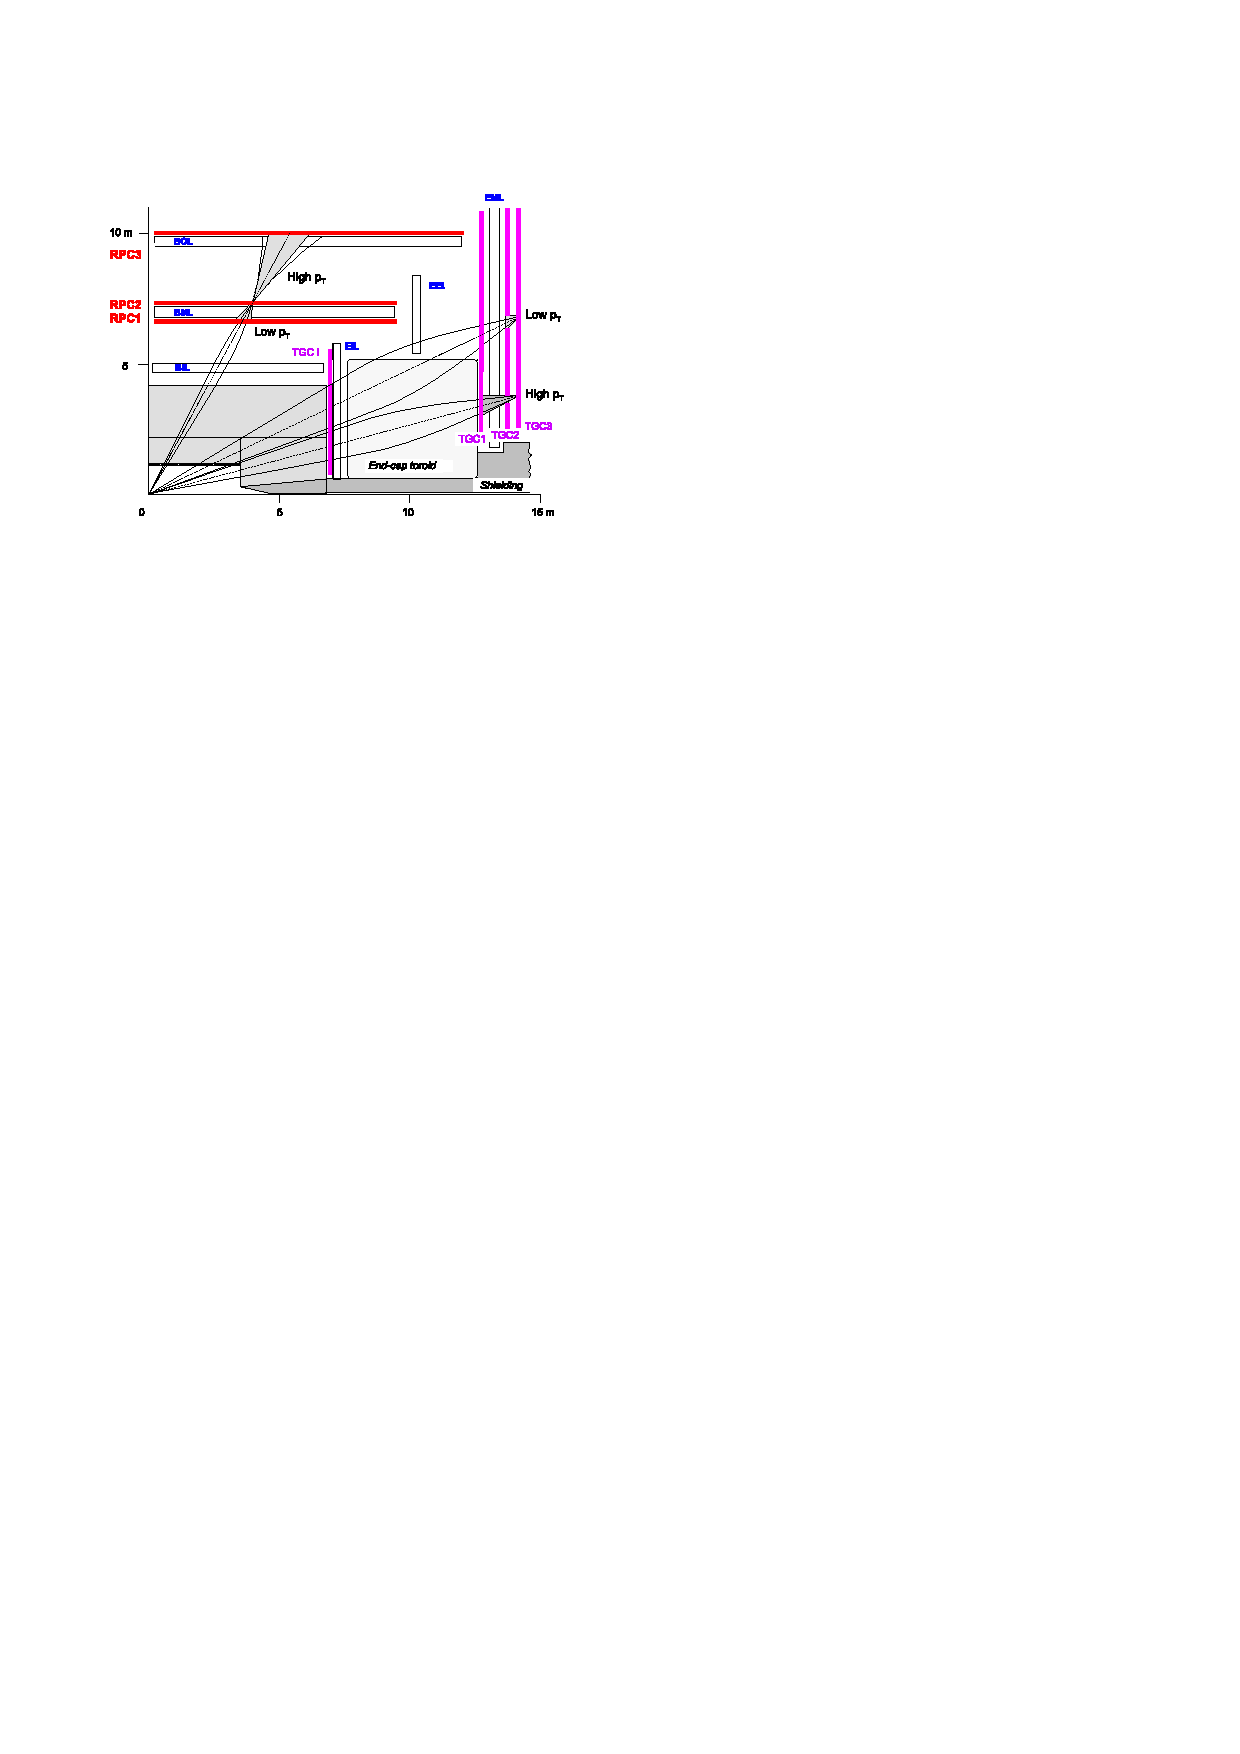
\includegraphics[width=0.8\textwidth]{mu-trigger-diag}
\caption{
Cross sectional view of the muon trigger chambers. Figure from~\cite{Aad:2012xs}.}
\label{fig:mu-trigger-diag}
\end{figure}

The muon HLT uses similar algorithms to the online muon reconstruction described
below. Each L1 muon candidate is refined by including the precision
data from the MDTs and CSCs in the RoI defined by the L1 candidate. MS tracks
are then built by opening narrow roads around the L1 trigger chamber hits and
associating hits from other chambers to the track. A rough \pt\ measurement is
obtained using a lookup table. The MS tracks are then combined with ID tracks,
reconstructed using the same fast L2 ID tracking as the electron L2 trigger
(see~\sec{reco-el-triggers}). The muon EF uses the full offline algorithms,
running in RoIs determined by the L2 trigger. There are two reconstruction
strategies used at EF level:
\intro{outside-in} (starting from the reconstructed MS tracks, extrapolating to
the IP and attempting to combine with an ID track) and \intro{inside-out}
(starting from ID tracks and attempting to extrapolate to the MS). In 2011, both
strategies were ran in parallel to maximise efficiency. In 2012, to reduce
processing time, the outside-in algorithm is run first, and only in events failing
the trigger at this stage is the inside-out algorithm run. In 2011 the offline
threshold used for the primary single muon trigger was 18 \GeV; in 2012 it was 24 \GeV. The muon trigger is
not very sensitive to pile-up, but modifications were required in 2012 in order
to keep the rate at an acceptable level in the higher luminosity conditions. To
achieve this a track based isolation cut was applied to EF level, requiring that
the sum of the \pt\ of tracks in a cone of \deltaRlt{0.2} around the muon track
be less than 12\% of the muon's \pt. Only tracks with \ptgt{1} enter the
calculation, and must have  $|\Delta z_{0}| <$ 6mm where $\Delta z_{0}$ is the
difference in transverse impact parameter between the track and the muon track.

\subsection{Reconstruction and Identification}
\label{sec:reco-el-reco}
